% !TeX spellcheck = en_US
\documentclass[letterpaper,12pt,twoside]{report}
\usepackage{fancyhdr}
\usepackage{fullpage}
\usepackage{tikz}
\usepackage{amsmath}

\begin{document}
	\pagestyle{fancy}
	\fancyhf{}
	\fancyhead[L]{Day 3}
	\fancyhead[R]{\textit{The Calendar Project}}
	\fancyfoot[L]{Citations Involved: 1, 2, 3}
	
	% Problem
	\paragraph{Problem}
	\begin{quote}
	\textsf{When all the diagonals in a regular hexagon are drawn, how many pairs of diagonals will be perpendicular?}
	\end{quote}
	
	% Graphics
	\begin{center}
		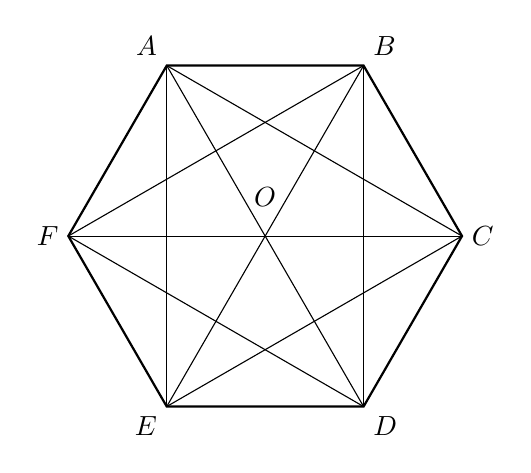
\begin{tikzpicture}[scale=0.5]
		\draw[thick] (5,0) -- (2.5,-4.33) -- (-2.5,-4.33) -- (-5,0) -- (-2.5,4.33) -- (2.5,4.33) -- cycle;
		\draw (5,0) -- (-2.5,4.33);
		\draw (5,0) -- (-5,0);
		\draw (5,0) -- (-2.5,-4.33);
		\draw (-5,0) -- (2.5,4.33);
		\draw (-5,0) -- (2.5,-4.33);
		\draw (-2.5,4.33) -- (-2.5,-4.33);
		\draw (-2.5,4.33) -- (2.5,-4.33);
		\draw (2.5,4.33) -- (-2.5,-4.33);
		\draw (2.5,4.33) -- (2.5,-4.33);
		
		\node[above left] at (-2.5,4.33) {$A$};
		\node[above right] at (2.5,4.33) {$B$};
		\node[right] at (5,0) {$C$};
		\node[below right] at (2.5,-4.33) {$D$};
		\node[below left] at (-2.5,-4.33) {$E$};
		\node[left] at (-5,0) {$F$};
		\node[above] at (0,0.5) {$O$};
		
		\end{tikzpicture}
	\end{center}
	
	% Reasoning
	\paragraph{Reasoning}
	\begin{quotation}
	
	The complement of the condition that \textit{``at least 1 six appears''} is that no six appears, which has a probability of $\frac{\textrm{\small{favorable}}}{\textrm{\small{all possible}}} = \frac{5}{6}$ for 1 roll (1). Since it is given that the die is tossed 6 times, and since this negated condition requires \textbf{all} rolls (not just one) to not be six, the cumulative probability for this negated condition is $(\frac{5}{6})^6 = \frac{5^6}{6^6} = \frac{15625}{46656}$ (3). This result's complement, the solution to the problem, is $1-\frac{15625}{46656} = \boxed{\frac{31031}{46656} \approx 0.665}$ (2).
	
	\end{quotation}
	
	\paragraph{External References}
	
	\begin{enumerate}
		\item Textbook Ch. 13, Pg. 878: Theoretical Probability
		\item Textbook Ch. 13, Pg. 879: Complement
		\item Textbook Ch. 13, Pg. 887: Probability of Independent Events
	\end{enumerate}

\end{document}